\chapter{Interface Design} % Main chapter title

\label{Chapter6} % For referencing the chapter elsewhere, use \ref{Chapter1} 

\lhead{Chapter 6. \emph{Interface Design}} % This is for the header on each page - perhaps a shortened title

%----------------------------------------------------------------------------------------
This section provides detailed illustration of the non-interactive
(map animation) and interactive dynamic energy map implementation and
design choices regarding the interactive dynamic energy map. The
section starts with a general overview that explains possible
approaches to add the time dimension in an energy map. Then the
non-interactive energy map (map animation) approach is presented. For
the non-interactive animation, the advantages and disadvantages
between different symbol or color representation on the effectiveness
of conveying information was briefly discussed.

Next a detailed documentation of the dynamic energy map interface is
presented. The layout and functions of each components of the
interface is explained and the design of each component based on
literature studies of dynamic map design is discussed. The use of
dynamic energy map to identify energy recovery opportunities and to
help design and size a district energy system is demonstrated.

\section{Overview}

Dorling and Openshaw pointed out that a dynamic map provides new
potential and possibilities for data analysis but also poses a great
challenge as a result of the less developed theory in space-time
pattern detection and measurement~\cite{Dorling1992}. In order to
better conduct a space-time visualization of the space-time energy
demand information in the dynamic energy map,literature studies on
space-time map visualization were used to design the dynamic energy
map.

Brownrigg mentions several methods of representing time on a map: 1) a
graph or chart that represents a function over time or a time line for
displaying chronological events 2) a sequence of snapshots displayed
over time (animated map) 3) small-multiples of snapshots of changing
states ~\cite{Brownrigg2005}.

Based on the classification above, method 1) and 2) were applied to
represent time for the dynamic energy map. The dynamic plot of
temporal time series uses method 1) to anchor the quantitative
information. The sequential map image display is using method 2). The
researcher did not use the small multiple method (method 3)). The
choice is based on the following points mentioned by Brownrigg: 1) the
number of snapshots in one display is limited and the finer the detail
per snapshot, the less snapshots one can contain in one display. Since
the 3D representation is chosen as one of the major map display
methods (2D map is also available), the level of details per image is
relatively high. This will result in a very small number of multiples
per display~\cite{Brownrigg2005} 2) the subtle changes are easier to
be noticed in the form of animation than with small-multiples
~\cite{Brownrigg2005}. Both drawbacks of small-multiple method will
impair the ability to convey the rapid temporal changes of community
energy behavior, hence is not suitable for the current project.

\section{(Non-interactive) Map Animation} \label{anime} 

Map animation was introduced to cartography in
1930s~\cite{Harrower2008}. Its major application include: 1)
demonstrating the dynamic process of geographic events (weather maps
in weather forecasting is such an example) 2) assisting pattern
recognition and knowledge development for scientific researches. The
study by Dorling and Openshaw is an example of application 2), where
they discovered new leukaemia hotspots through animated
maps~\cite{Dorling1992}.  Animated maps are proven to be more powerful
in conveying the spatial-temporal pattern than static
maps~\cite{McEachern1998}.

The level of user control of playback behavior of animated maps is
debatable. Providing the full freedom of adjusting the playback can
enhance pattern understanding~\cite{Nelson1998}, but it might also
reduce time animation to still images and impair its ability in
conveying temporal changes ~\cite{Lowe2004}. In the current dynamic
map project. The researcher observed that the non-interactive map
animation is especially helpful in conveying the dynamic energy
changing and the non-coincident peak arriving time of different
buildings in the community. Resch et al.\ suggest that the interface
for general public should ``ensure that the amount of information
shown to the users at any given time, and its complexity, are
reduced''~\cite{Resch2014}. The non-interactive animated map could be
one of the potential choices for an interface of a dynamic energy map
with general public as the target user group.

For this project a continuous color encoding method was used in the
creation of non-interactive animation of a univariate gas heating
energy demand map. Similar to the National Heat Map, the Calgary Map
and the EMIOFN project (\tref{tab:mapRep}) discussed in
\sref{sec:mapRepre}, a red to blue color ramp is used in the map
display. Different from the cases above, the current project chose to
represent high heat demand with blue and low heat demand with red as a
result of a limited survey of potential users. Each color within this
red-to-blue color scheme is represented as a real number between 0 and
1 with 0 representing pure red and 1 representing pure blue.

The first approach to calculate the corresponding color for each
heating energy value is to calculate the normalized distance between
the current value and the maximum value (\eref{eq:linear}).

\begin{equation}\label{eq:linear}
  {E(t) – E_{max} \over E_{max}}
\end{equation}

$E(t)$ is the energy consumption for the current time spot $t$,
$E_{max}$ is the maximum energy consumption over the year. The problem
for this approach is that the color changing is not visible enough as
a result of a extremely right skewed energy data (with each data point
representing the hourly energy consumption of a certain building in
the community at a certain hour of a year) distribution
(\fref{fig:heatOri}).

\begin{figure}[h!]
  \centering
  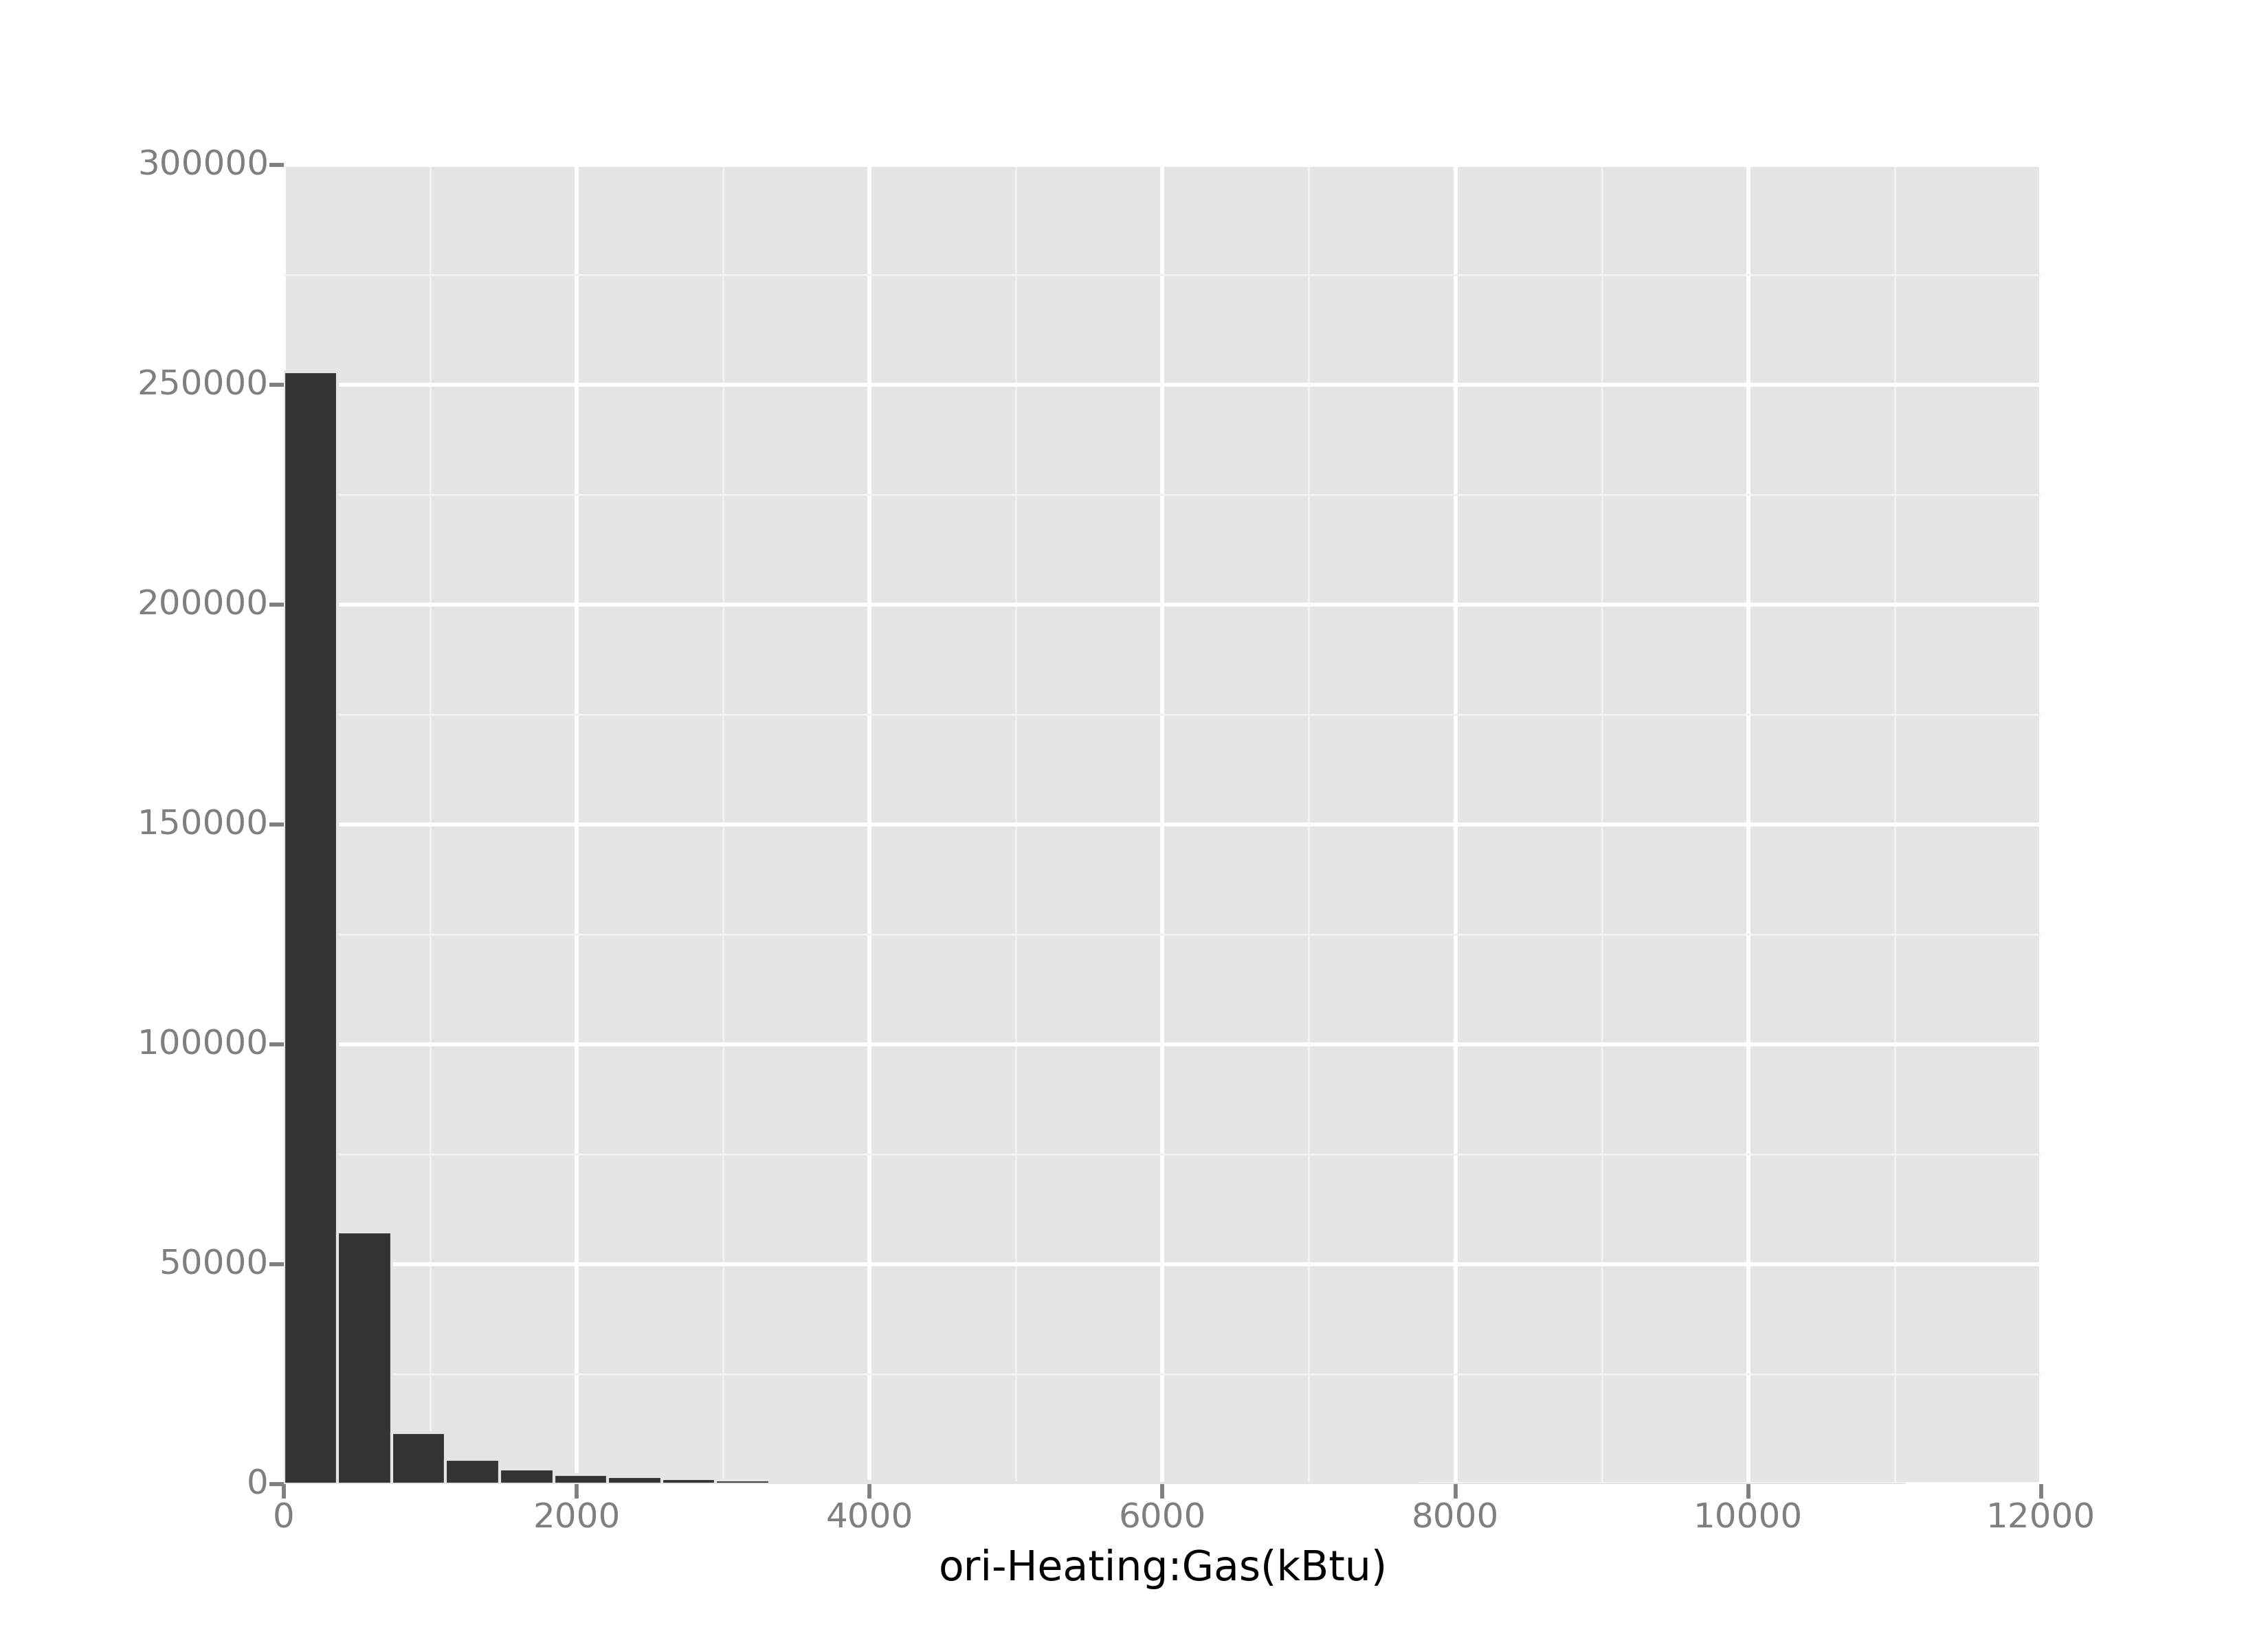
\includegraphics[width=0.7\linewidth]{heatOri.png}
  \caption[Heating Demand Histogram of Conceptual City]{A histogram of
    hourly energy consumption per building, for the 68 buildings in
    the community}
  \label{fig:heatOri}
\end{figure}

By directly applying this normalized color scheme, the color
distribution on a map will be very un-even, with most of the buildings
colored with the red color for most of the time.

Kolter and Ferreira discovered that the annual total energy
consumption of the 6500 buildings in Cambridge MA area follows a
``log-normal'' distribution~\cite{Zico2011}. By applying similar log
scaling for the hourly heating energy data of the community, we found
that the hourly heating energy distribution also roughly follows a
normal distribution (\fref{fig:heatLog}). We apply log scaling to
flatten the distribution and calculate the color from energy
($E(t)$) as follows:

\begin{equation}\label{eq:log}
  {\ln(E(t)) – \ln(E_{max}) \over \ln(E_{max})}
\end{equation}

\begin{figure}[h!]
  \centering
  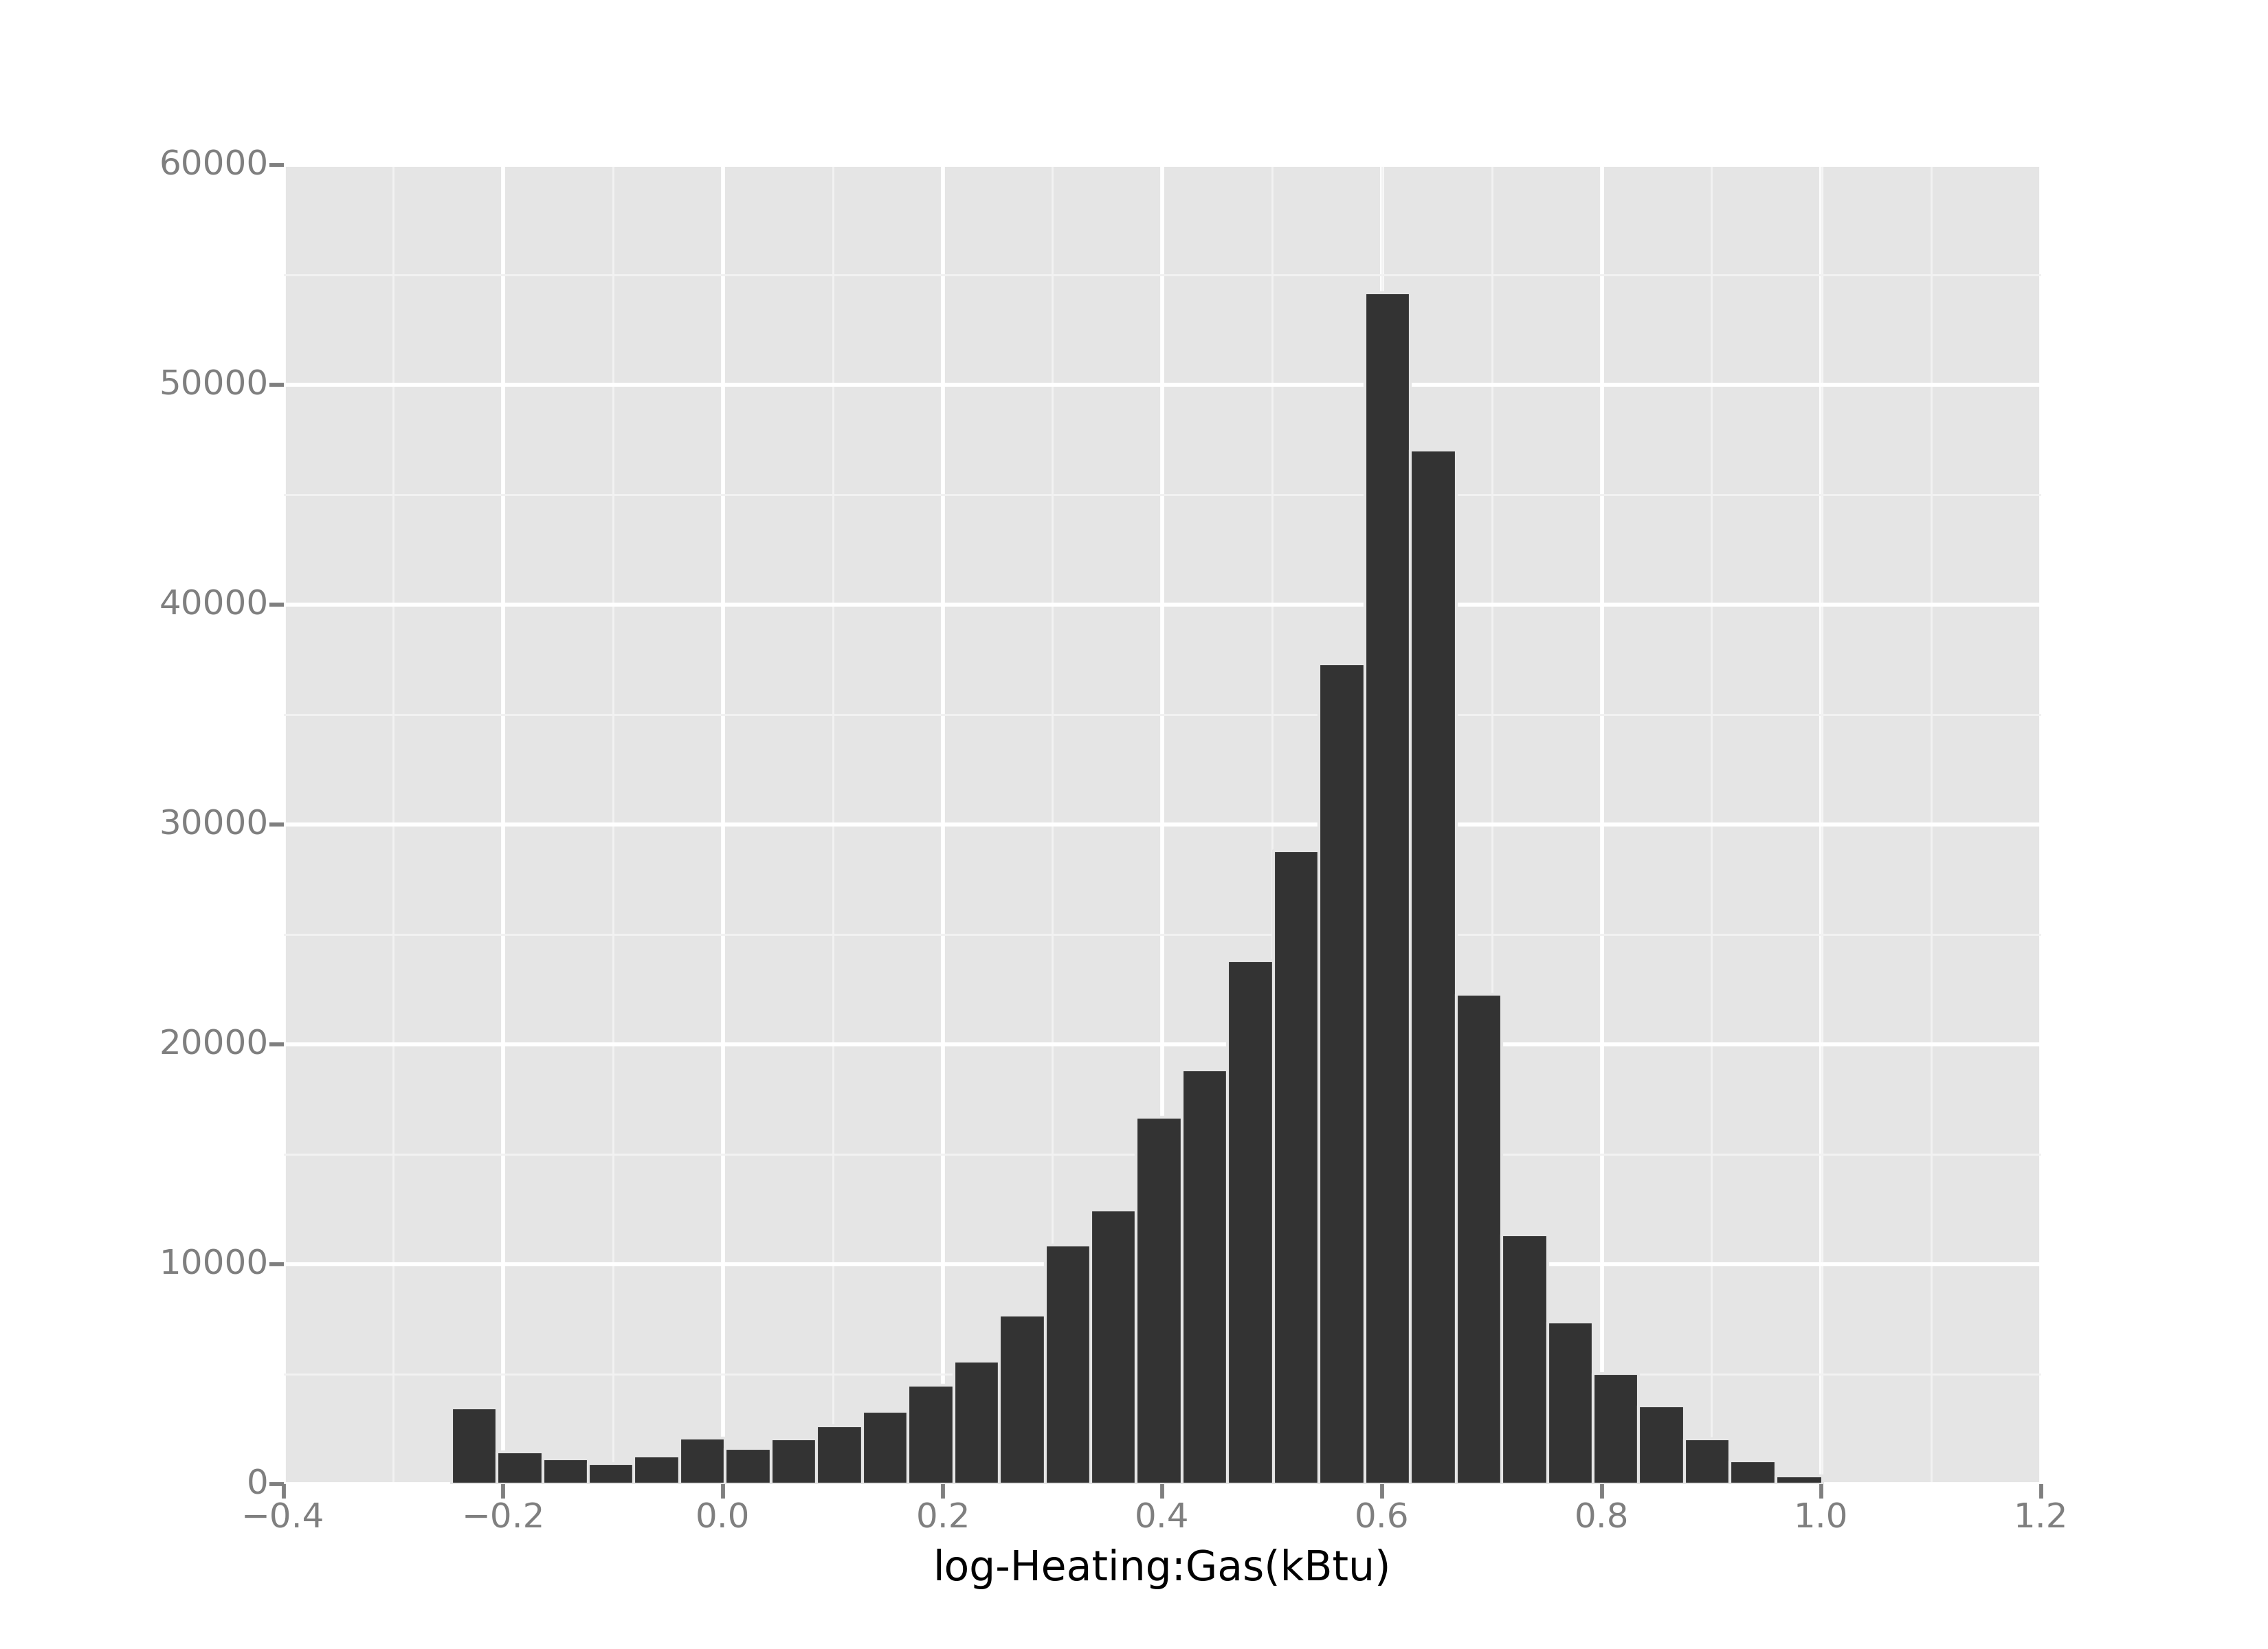
\includegraphics[width=0.7\linewidth]{heatLog.png}
  \caption[Heating Demand of Conceptual City]{Heating Demand of
    Conceptual City}
  \label{fig:heatLog}
\end{figure}

\fref{fig:img0002} is one snapshot of the conceptual urban environment
model under the log scaled calculation method in \eref{eq:log}.
\begin{figure}[h!]
  \centering
  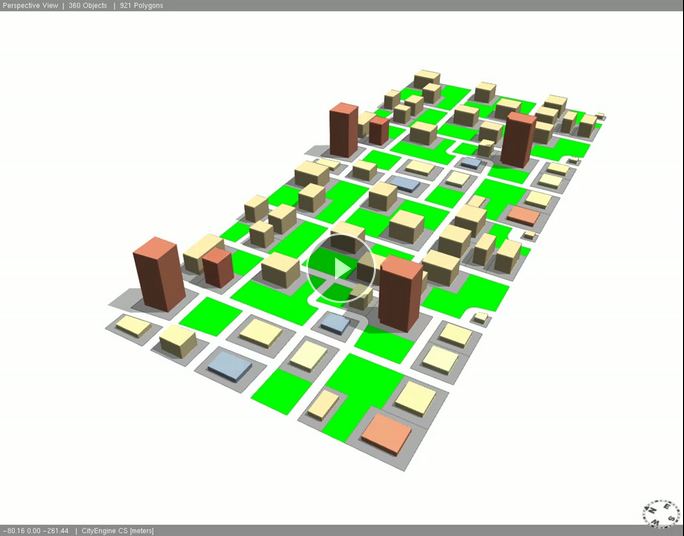
\includegraphics[width=0.7\linewidth]{img0002.png}
  \caption[Animation Demo of the Color Calculation]{Animated
    demonstration of the log-scaled dynamic energy heating demand map}
  \label{fig:img0002}
  \href{http://www.armechxyj.com/energy-mapping.html/#colorAnime}{Click
    here to go to the animation link}.
\end{figure}

In the dynamic energy map interface design, the researcher applied a
discrete color encoding with a seven-class bivariate choropleth
representation (\tref{tab:breakpoint}). The break points are
calculated purely with the Quantile method in
\sref{dataClassification}. This allows for a quantitative legend that
can depict more specific energy demand information. An animation with
this discrete color scheme is also created and can be viewed and
downloaded
\href{http://www.armechxyj.com/energy-mapping.html#redblueAnime3d}{through
  this link}.

\begin{table}[]
\centering
\caption{Heating-Cooling Breakpoints in the Interface}
\label{tab:breakpoint}
\begin{tabular}{rr|rr}
  \hline
heating &      & cooling &     \\
  \hline
  \hline
kBtu    & Ton  & kBtu    & Ton \\
5       & 60   & 2       & 24  \\
22      & 264  & 7       & 84  \\
50      & 600  & 15      & 180 \\
91      & 1092 & 26      & 312 \\
136     & 1632 & 56      & 672 \\
213     & 2556 & 72      & 864\\
  \hline
\end{tabular}
\end{table}

Although the initial conditions of the map instances using the
continuous and discrete encoding method are different: the animation
with continuous color encoding depicts only one variable (gas heating)
while the animation with discrete color encoding depicts two variables
(space heating and cooling), the researcher observed that the
continuous color encoding method seems to be better in demonstrating
the general pattern of energy changing behavior. Further evaluations
are needed to compare these two approaches and justify the design
choice of a discrete or continuous color scheme.

\begin{comment}
\section{Future Trends}
Harrower and Fabrikant mentioned that the chanllenge of using animated
maps is the overflow of information and the vulnerability to
distraction~\cite{Harrower2008}. One example mentioned by Harrower and
Fabrikant is the comparison of color on the map and that on the legend
becomes difficult for animated maps as a result of the changing of
images. They proposed the audio legend approach of strengthening
information convey with minimized
distraction~\cite{Harrower2008}. This might become one of the next
extensions of the current Dynamic Energy Map interface design.

They also suggested that the difference in time should have different
visual representations in data display~\cite{Harrower2008}. Peuquet
claimed that ``The development of temporal analytical capabilities in
GIS such as temporal queries requires basic topological structures in
both time and space''~\cite{Peuquet1994}. Thus the different spatial
representation seems to be a natural choice for adapting to different
temporal resolution and scale.


The non-interactive animation could be found
\href{http://www.armechxyj.com/energy-mapping.html#redblueAnime3d}{through
  this link}.
\end{comment}